\documentclass[10pt]{mypackage}

% sans serif font:
%\usepackage{cmbright,sfmath,bbold}
%\renewcommand{\mathcal}{\mathtt}

%Euler:
\usepackage{newpxtext,eulerpx,eucal,eufrak}
\renewcommand*{\mathbb}[1]{\varmathbb{#1}}
\renewcommand*{\hbar}{\hslash}
\newcommand{\ds}{\displaystyle}
\DeclareMathOperator{\Ln}{Ln}
\DeclareMathOperator{\Arg}{Arg}
\DeclareMathOperator{\Arctan}{Arctan}
\DeclareMathOperator{\Res}{Res}
\DeclareMathOperator{\res}{Res}

%\usepackage{homework}

\pagestyle{fancy} %better headers
\fancyhf{}
\rhead{Avinash Iyer}
\lhead{Mathematical Methods II Notes}

\setcounter{secnumdepth}{0}

\begin{document}
\RaggedRight
\section{Complex Analysis}%
\subsection{Analyticity and Path-Independence in the Complex Plane}%
\subsubsection{Baby's First Complex Function Theory}%
We are interested in functions of the form $f(z)$, where $z = x+iy$ is some complex number. Note that this is specifically different from a function $g\colon \R^2\rightarrow \Omega$ for some domain $\Omega$; in the latter case, we have independent variables $x$ and $y$, while in the former case, we must express $z = x+iy$.\newline

Now, consider a contour integral
\begin{align*}
  \oint_{C}^{} w(z)\:dz &= \oint_{C}w(z)\:\left(dx + idy\right)\\
                        &= \oint_{C}^{} w(z)\:dx + i\oint_{C}w(z)\:dy.
                        \intertext{Taking $A_x = w(z)$ and $A_y = iw(z)$, we have}
                        &= \oint_{C}^{} \mathbf{A}\cdot\:d\vec{\ell}.
                  \intertext{We want to know if this is equal to, by Green's Theorem,}
                        &= \int_{S}^{} \left(\nabla\times \mathbf{A}\right)\:d\mathbf{a},
\end{align*}
and when this integral is zero. Note that $\left(\nabla\times \mathbf{A}\right)\cdot \hat{n} = 0$, so $\pd{A_y}{x} - \pd{A_x}{y} = 0$.\newline

Note that we can take
\begin{align*}
  w(z) &= u(x,y) + iv(x,y),
\end{align*}
where $z = x + iy$.\newline

After a lot of tedious derivation, we get the Cauchy--Riemann equations.
\begin{theorem}[Cauchy--Riemann Equations]
  \begin{align*}
    \pd{u}{x} &= \pd{v}{y}\\
    \pd{v}{x} &= -\pd{u}{y}.
  \end{align*}
\end{theorem}
Furthermore, the Cauchy--Riemann equations guarantee that $w$ is analytic,\footnote{Equal to its Taylor series, also holomorphic.} which leads to Cauchy's theorem.
\begin{theorem}[Cauchy's Theorem]
  If $C$ is a simple closed curve in a simply connected region, then $w$ is analytic if and only if
  \begin{align*}
    \oint_{C}^{} w(z)\:dz &= 0.\label{thm:cauchy_integral_thm}\tag{\textdagger}
  \end{align*}
\end{theorem}
\begin{fact}
The function $w(z)$ is analytic inside the simply connected region $R$ if any of these hold:
\begin{itemize}
  \item $w$ satisfies the Cauchy--Riemann equations;
  \item $w'(z)$ is unique and exists;
  \item $\pd{w}{\overline{z}} = 0$.
  \item $w$ can be expanded as $w(z) = \sum_{n\geq 0}c_n\left( z-a \right)^n$, convergent on some open neighborhood of $a$ for each $a$ on its domain;\footnote{This is technically the real definition of analytic for the case when we're dealing with a function with domain $\R$.}
  \item $w(z)$ is path-independent everywhere in $R$: $\oint_{C}w(z)\:dz = 0$.
\end{itemize}
\end{fact}
\begin{example}
  Considering $w(z) = z$, we have $u=x$ and $v=y$, so it satisfies the Cauchy--Riemann equations. However, neither $\re\left(z\right)$ nor $\im\left(z\right)$ are analytic, and neither is $\overline{z} = x-iy$.
\end{example}
\begin{remark}
Whenever we say ``analytic at $p$,'' we mean ``analytic in a neighborhood of $p$.''
\end{remark}
Note that since $\C$ is a non-compact locally compact Hausdorff space, we may carry out a one-point compactification of $\C$, by adjoining a point $\set{\infty}$, $\C^{\ast} = \C\cup \set{\infty}$. This compactified $\C^{\ast}$ is often represented as a unit sphere with the north pole, determined by $\left(0,0,1\right)$, is the point at infinity. The correspondence between $\C^{\ast}\setminus\set{\infty}$ and $\C$ is evaluated via stereographic projection.\newline

We define $\frac{z}{\infty} = 0$ and $\frac{z}{0} = \infty$ for any $z\neq 0,\infty$. The correspondence between $z = x + iy$ in the plane to $Z$ on the Riemann sphere with $\R^3$ coordinates $\left(\xi_1,\xi_2,\xi_3\right)$ is
\begin{align*}
  \xi_1 &= \frac{2\re(z)}{\left\vert z \right\vert^2 + 1}\\
  \xi_2 &= \frac{2\im\left(z\right)}{\left\vert z \right\vert^2 + 1}\\
  \xi_3 &= \frac{\left\vert z \right\vert^2 - 1}{\left\vert z \right\vert^2 + 1}.
\end{align*}
Inverting, we may find
\begin{align*}
  x &= \frac{\xi_1}{1-\xi_3}\\
  y &= \frac{\xi_2}{1-\xi_3},
\end{align*}
and with polar coordinates,
\begin{align*}
  z &= \cot\left(\theta/2\right)e^{i\phi}.
\end{align*}

\begin{center}
  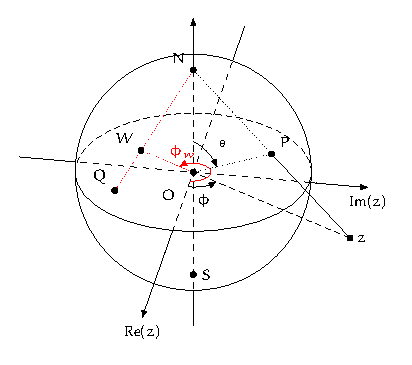
\includegraphics[width=7cm]{images/riemann_sphere.pdf}
\end{center}
To determine analyticity at $\infty$, we set $\zeta = \frac{1}{z}$, and analyze the analyticity of $\tilde{w}\left(\zeta\right) = w\left(1/z\right)$ at $0$.
\subsubsection{Cauchy's Integral Formula}%
Consider the function $w(z) = c/z$, integrated around a circle of radius $R$. Then, writing $z = Re^{i\varphi}$, we get
\begin{align*}
  \oint_{\Gamma}w(z)\:dz &= C\int_{0}^{2\pi} \frac{e^{-i\varphi}}{R}\underbrace{iRe^{i\varphi}\:d\varphi}_{dz}\\
                         &= ic\int_{0}^{2\pi} \:d\varphi\\
                         &= 2\pi i c.
\end{align*}
If our contour $C$ runs around our singularity at $z = 0$ a total of $n$ times, then we pick up a factor of $n$.\newline

Now, when we consider
\begin{align*}
  I &= \oint_{C}\frac{dz}{z^n},
\end{align*}
this integral actually yields $0$ for any $n\neq 1$, despite the fact that $0$ is a singularity for $f(z) = \frac{1}{z^n}$. This $0$ is not a reflection of \hyperref[thm:cauchy_integral_thm]{Cauchy's integral theorem}, but of the fact that
\begin{align*}
  z^{-n} &= \frac{d}{dz}\left(\frac{z^{-n+1}}{n+1}\right),
\end{align*}
meaning that $z^{-n}$ is an exact differential, so integrating along a closed curve yields zero change. However, $\frac{1}{z} = \diff{}{z}\left(\ln z\right)$ may be an exact differential, but for complex $z$, $\ln z = \ln\left\vert z \right\vert + i\arg(z) = \ln r + i\varphi$. This yields
\begin{align*}
  \oint_{C} \frac{c}{z}dz &= c\oint_{C} d\left(\ln z\right)\\
                          &= c\left(i\left(\varphi + 2\pi\right) - \varphi\right)\\
                          &= 2\pi i c.
\end{align*}
Ultimately, what this shows is that when we integrate any analytic function $f\left(\zeta\right)$ along a closed contour with a singularity at $z$, only the coefficient on $\frac{1}{\zeta -z}$ will remain. This coefficient is known as the residue at $0$.
\begin{theorem}[Cauchy's Integral Formula]
  If $w$ is analytic in a simply connected region and $C$ is a closed contour winding once around a point $z$ in the region, then
  \begin{align*}
    w(z) &= \frac{1}{2\pi i} \oint_{C}\frac{w\left(\zeta\right)}{\zeta - z}\:d\zeta.\label{thm:cauchy_integral_formula}\tag{\textasteriskcentered\textasteriskcentered}
  \end{align*}
\end{theorem}
Furthermore, this shows that any once-differentiable function is infinitely differentiable, as by differentiating under the integral sign, we get
\begin{align*}
  \diff{^nw}{z^n} &= \frac{n!}{2\pi i} \oint_{C} \frac{w\left(\zeta\right)}{\left(\zeta - z\right)^{n+1}}\: d\zeta.
\end{align*}
\begin{example}[Deriving Liouville's Theorem]
  Consider a circle $C$ centered at radius $r$ centered at at $z$, $\zeta - z = Re^{i\varphi}$. We take $d\zeta = iRe^{i\varphi}\:d\varphi$, and taking derivatives, we have
  \begin{align*}
    w'(z) &= \frac{1}{2\pi R} \int_{0}^{2\pi} w\left(z + Re^{i\varphi}\right)e^{-i\varphi}\:d\varphi.
  \end{align*}
  If $w$ is bounded --- i.e., $\left\vert w(z) \right\vert \leq M$ for all $z$ in a given region --- then
  \begin{align*}
    \left\vert w'(z) \right\vert &= \left\vert \frac{1}{2\pi R} \int_{0}^{2\pi} w\left(z + Re^{i\varphi}\right)e^{-i\varphi}\:d\varphi \right\vert\\
                                 &\leq \frac{1}{2\pi R} \int_{0}^{2\pi} \left\vert w\left(z + Re^{i\varphi}\right) \right\vert\:d\varphi\\
                                 &\leq \frac{M}{R}
  \end{align*}
  for all $R$ within the analytic region.\newline

  In the case where $w$ is entire (i.e., analytic on $\C$), then this inequality holds for all $R\rightarrow\infty$. Thus, $\left\vert w'(z) \right\vert = 0$ for all $z$, meaning that $w$ is constant.\newline

  This is known as Liouville's theorem --- every bounded entire function is constant. This can be used to prove the fundamental theorem of algebra.\newline

  What Liouville's theorem tells us is that any nontrivial behavior will emerge from a function's singularities.
\end{example}
\subsection{Singularities and Branches}%
To understand nontrivial behavior on the complex plane, we need to understand singularities. This will require us to develop understanding of Laurent series.
\subsubsection{Taylor Series}%
We want to integrate $w(z)$ around some point $a$ in an analytic region of $w(z)$. This yields the form
\begin{align*}
  w(z) &= \frac{1}{2\pi i} \oint_{C}^{} \frac{w\left(\zeta\right)}{\zeta - z}\:d\zeta\\
       &= \frac{1}{2\pi i} \oint_{C} \frac{w\left(\zeta\right)}{\left(\zeta - a\right)-\left(z-a\right)}\:d\zeta\\
       &= \frac{1}{2\pi i} \oint_{C} \frac{w\left(\zeta\right)}{\left(\zeta - a\right)\left(1 - \frac{z-a}{\zeta - a}\right)}\:d\zeta.\label{step:geometric_expansion}\tag{\textdaggerdbl}
       \intertext{Since $\zeta$ is on the contour and $z$ is in the contour, $\left\vert \frac{z-a}{\zeta - a} \right\vert < 1$, we may expand as a geometric series. Thus, we get}
       &= \frac{1}{2\pi i} \oint_{C} \frac{w\left(\zeta\right)}{\left(\zeta - a\right)}\left(\sum_{n=0}^{\infty}\left(\frac{z-a}{\zeta - a}\right)^{n}\right)\:d\zeta.
       \intertext{Since the series is uniformly convergent, we are allowed to exchange sum and integral, yielding}
       &= \sum_{n=0}^{\infty}\underbrace{\left(\frac{1}{2\pi i}\oint_{C}\frac{w\left(\zeta\right)}{\left(\zeta - a\right)^{n+1}}\:d\zeta\right)}_{=c_n} \left(z-a\right)^n\\
       &= \sum_{n=0}^{\infty}c_n\left(z-a\right)^n,
       \intertext{where}
  c_n &= \frac{1}{n!} \left.\diff{^nw}{z^n}\right|_{z=a}.
\end{align*}
If our Taylor series reduces to a known series on the real axis, we find this very desirable. We say this is a type of analytic continuation from the real axis to the complex plane. For example,
\begin{align*}
  e^z &= \sum_{k=0}^{\infty}\frac{z^k}{k!}
\end{align*}
is an analytic continuation of $e^x$.\newline

However, more interestingly,
\begin{align*}
  \zeta\left(s\right) &= \sum_{k=1}^{\infty}\frac{1}{k^s}
\end{align*}
converges for all $s > 1$. However, we have also shown that
\begin{align*}
  \zeta\left(s\right) &= \frac{1}{\Gamma(s)}\int_{0}^{\infty} \frac{x^{s-1}}{e^{x}-1}\:dx
\end{align*}
converges for complex $s$ for all real part greater than $1$. Since values of this integral agree with the series representation of $\zeta(s)$ on real axis, we have that this is an analytic continuation of $\zeta(s)$ to the subset of $\C$ defined by $\re(s) > 1$.
\subsubsection{Laurent Series}%
Now, what happens if, at \eqref{step:geometric_expansion}, we have $\left\vert \frac{z-a}{\zeta - a} \right\vert > 1$. The series as constructed would not converge, but what if we have a series that converges everywhere \textit{outside} $C$? This would entail an expansion in reciprocal integer powers of $z-a$. This yields
\begin{align*}
  w(z) &= -\frac{1}{2\pi i} \oint_{C}\frac{w\left(\zeta\right)}{\left(z-a\right)\left(1-\frac{\zeta - a}{z-a}\right)}\:d\zeta\\
       &= -\frac{1}{2\pi i} \oint_{C} \frac{w\left(\zeta\right)}{z-a}\left(\sum_{n=0}^{\infty}\left(\frac{\zeta - a}{z-a}\right)^n\right)\:d\zeta\\
       &= -\sum_{n=0}^{\infty}\left(\frac{1}{2\pi i}\oint_{C}w\left(\zeta - a\right)^n\:d\zeta\right)\frac{1}{\left(z-a\right)^{n+1}}\\
       &= \sum_{n=1}^{\infty}\underbrace{\left(-\frac{1}{2\pi i}\oint_{C}w\left(\zeta - a\right)^{n-1}\:d\zeta\right)}_{=c_{-n}}\frac{1}{\left(z-a\right)^{n}}\\
       &= \sum_{n=1}^{\infty}\frac{c_{-n}}{\left(z-a\right)^n}
\end{align*}
Note that this series has a singularity at $z = a$, but since our series is only defined outside a particular region, that doesn't matter. We call a series in reciprocal powers a Laurent series. More specifically, Laurent series may include expansions in negative powers as well as positive powers.
\begin{example}[Annuli]
  If we have a point $a$, we want to surround $a$ by a special contour to apply Cauchy's integral formula.\newline

  In particular, for any $z$ in the annulus, we get
  \begin{align*}
    w(z) &= \frac{1}{2\pi i} \oint_{c_1 - c_2}^{} \frac{w\left( \zeta \right)}{\zeta - z}\:d\zeta\\
         &= \frac{1}{2\pi i} \oint_{c_1}^{} \frac{w\left( \zeta \right)}{\zeta - z}\:d\zeta - \frac{1}{2\pi i}\oint_{c_2}^{} \frac{w\left( \zeta \right)}{\zeta - z}\:d\zeta\\
         &= \sum_{n=-\infty}^{\infty}c_n\left( z-a \right)^n\\
         &= c_0 + \sum_{n=1}^{\infty}\left( c_{-n}\left( z-a \right)^n + c_n\left( z-a \right)^n \right).
  \end{align*}
\end{example}
\begin{example}
  Consider the function
  \begin{align*}
    w(z) &= \frac{1}{z^2 + z - 2}\\
         &= \frac{1}{\left( z- 1\right)\left( z+2 \right)}\\
         &= \frac{1}{3}\left( \frac{1}{z-1} - \frac{1}{z+2} \right).
  \end{align*}
  Now, we have three regions to expand $w$ in.
  \begin{itemize}
    \item If $\left\vert z \right\vert < 1$, then our series is in both $\displaystyle z^n$ and $\displaystyle z^n$.
    \item If $1 < \left\vert z \right\vert < 2$, then one of our series is going to in $\displaystyle \frac{1}{z^{n}}$ and one is in $\displaystyle z^n$.
    \item If $\left\vert z \right\vert > 2$, then both of our series are in the form of $\displaystyle \frac{1}{z^n}$ and $\displaystyle \frac{1}{z^n}$
  \end{itemize}
  Via tedious, heavily error-prone calculations, we find that
  \begin{align*}
    w_1(z) &= -\frac{1}{3}\sum_{n=0}^{\infty}\left( 1 + \left( -1 \right)^n \left( \frac{1}{2} \right)^{n+1} \right)z^n\\
    w_2(z) &= \frac{1}{3}\sum_{n=0}^{\infty}\left( \frac{1}{z^{n+1}} + \left( -\frac{1}{2} \right)^{n+1}z^n \right)\\
    w_3(z) &= \frac{1}{3} \sum_{n=0}^{\infty} \left( 1-\left( -2 \right)^n \right)\frac{1}{z^{n+1}}.
  \end{align*}
  Sewing all of $w_1,w_2,w_3$ together, then we get a full series representation of $w(z)$.
\end{example}
\begin{definition}
  If $w(z)$ is a function that can be written as $w(z) = \left( z-a \right)^ng(a)$, where $g(a)\neq 0$, then we say $w$ has an $n$-th order zero at $z=a$. If $n = 1$, then we say $w$ has a simple zero at $a$.\newline

  Similarly, if we can write
  \begin{align*}
    w(z) &= \frac{g(a)}{\left( z-a \right)^n}
  \end{align*}
  with $g(a)\neq 0$, then we say $w$ has a pole of order $n$ at $a$. If $n = 1$, then we say $w$ has a simple pole at $a$.
\end{definition}
There are three types of isolated singularities (i.e., isolated points where $w(z)$ is not defined).
\begin{definition}
  Let $w$ be an analytic function with isolated singularity at $a$.
  \begin{itemize}
    \item If $w$ remains bounded in any neighborhood of $a$, then it must be the case that $c_{-n} = 0$ for all $n > 1$, so the Laurent series is a pure Taylor expansion. We say $z = a$ is a removable singularity.\newline

      For instance, the function
      \begin{align*}
        \frac{\sin\left( z-a \right)}{z-a} &= \sum_{n=0}^{\infty}\left( -1 \right)^n \frac{\left( z-a \right)^{2n}}{\left( 2n+1 \right)!}
      \end{align*}
      has a removable singularity at $z=a$.
    \item If not all the $c_{-n}$ are equal to zero, but there is a largest $n > 0$ such that $c_{-n}$ is in the Laurent series expansion, then we say $a$ is an $n$-th order pole. If $n = 1$, we say $a$ is a simple pole.
    \item If there is no largest value of $n$ such that $c_{-n}$ is in the Laurent series --- i.e., that $c_{-n}\neq 0$ for all $n$ --- then we say that $a$ is an essential singularity.\newline

      One of the most important facts about an essential singularity is that the behavior is path dependent. For instance,
      \begin{align*}
        e^{1/z} &= \sum_{n=0}^{\infty}\frac{1}{n!z^n}
      \end{align*}
      has an essential singularity at $z = 0$. We see that $e^{1/z}$ diverges as $z \rightarrow 0$ along the positive real axis, but if $z\to 0$ along the negative real axis, we get $e^{1/z}\to 0$.
  \end{itemize}
  Singularities can also occur at $\infty$, which occurs when $w(1/z)$ has a singularity at $0$.
\end{definition}
\subsubsection{Multivalued Function}%
Consider the function
\begin{align*}
  w(z) &= z^2\\
       &= \underbrace{\left( x^2 - y^2 \right)}_{u(x,y)} + i\underbrace{\left( 2xy \right)}_{v(x,y)}\\
       &= r^2e^{2i\varphi}.
\end{align*}
Note that if we take a path around the origin going around by an angle of $2\pi$, then the resulting path goes around twice. Note that this means the lines $\varphi$ and $\varphi + \pi$ map to the same point in the $w$ plane.\newline

This isn't such a big deal in and of itself, but if we take $w(z) = z^{1/2}$, we get an issue. Instead of $w$ being a two-to-one function, we now have $w$ is a one-to-two function. This is an implicit problem in $\R$ with the function $w(x) =\sqrt{x}$, which we resolve by taking the ``positive'' square root. This is known as choosing a branch.\newline

We have to do something similar in the complex plane. Note that if we go around by an angle of $2\pi$ in the $z$ plane, then we only go around by an angle of $\pi$ in the $w$-plane. As we keep going around the plane, we jump from branch to branch, which brings issues of continuity.\newline

To resolve this, we create a ``branch cut'' that contours are not allowed to cross. 
\begin{example}
  The most common branch cut is to start from the branch point at $z = 0$, in the case of $w(z) = z^{1/2}$ or $w(z) = \ln(z)$, and extend along the real axis, meaning our branch cut is $\left( -\infty,0 \right]$.\newline

  This principal branch restricts \textit{output} values of $\varphi$ to $-\pi < \varphi \leq \pi$.\newline

  For instance, above the cut, we have $\varphi = \pi$, and below the branch cut, we have $\varphi = -\pi$, meaning we have
  \begin{align*}
    \sqrt{z} &= \sqrt{r}e^{i\pi /2}\tag*{$\varphi \to \pi$}\\
             &= i\sqrt{r}\\
    \sqrt{z} &= \sqrt{r}e^{-i\pi/2}\tag*{$\varphi \to -\pi$}\\
             &= -i\sqrt{r}.
  \end{align*}
  This is why the branch cut ``causes'' a discontinuity across the branch, but in $\C\setminus (-\infty,0]$.\newline

  Now, if we have
  \begin{align*}
    \sqrt{z_1}\sqrt{z_2} &= \left( r_1e^{i\varphi_1} \right)^{1/2}\left( r_2e^{i\varphi_2} \right)^{1/2}\\
                         &= \sqrt{r_1r_2}e^{i\left( \varphi_1 + \varphi_2 \right)/2}.
  \end{align*}
  However, if we want to calculate $\sqrt{z_1z_2}$, and if $\left\vert \varphi_1 + \varphi_2 \right\vert > \pi$ < then our product $z_1z_2$ crosses the branch cut, and our discontinuity requires $\varphi_1 + \varphi_2 $ to be converted to $\varphi_1 + \varphi_2 \pm 2\pi$ so as to bring the angle sum back into the principal branch. This means we have
  \begin{align*}
    \sqrt{z_1z_2} &= \left( r_1r_2e^{i\left( \varphi_1 + \varphi_2 \right)/2} \right)\\
                  &= \begin{cases}
                    \sqrt{r_1r_2}e^{i\left( \varphi_1 + \varphi_2 \right)/2} & \left\vert \varphi_1 + \varphi_2 \right\vert \leq \pi\\
                    -\sqrt{r_1r_2}e^{i\left( \varphi_1+\varphi_2 \right)/2} & \left\vert \varphi_1 + \varphi_2 \right\vert > \pi
                  \end{cases}.
  \end{align*}
\end{example}
\begin{example}
  Now, if we have $z_1 = 2e^{i\left( 3\pi/4 \right)}$ and $z_2 = e^{i\left( \pi/2 \right)}$, then we have
  \begin{align*}
    \sqrt{z_1} &= \sqrt{2}e^{i3\left( \pi/8 \right)}\\
    \sqrt{z_2} &= e^{i\left( \pi/4 \right)}.
  \end{align*}
  Note that if we take $\sqrt{z_1z_2}$, then the argument of $z_1z_2$ is $5\pi/4$, so we have to change our argument to $-3\pi/4$ to return to the principal branch before we may calculate the square root. This gives
  \begin{align*}
    \sqrt{z_1z_2} &= \sqrt{2e^{-i\left( 3\pi/4 \right)}}\\
                  &= \sqrt{2}e^{-i\pi + i\left( 5\pi/8 \right)}\\
                  &= -\sqrt{2}e^{i\left( 5\pi/8 \right)}\\
                  &= -\sqrt{z_1}\sqrt{z_2}.
  \end{align*}
\end{example}
Now, it is possible to have a branch point at $\infty$, by determining if $w\left( \frac{1}{z} \right)$ has a branch point at zero. For instance, if $w = z^{1/2}$, this gives
\begin{align*}
  w\left( \frac{1}{z} \right) &= \frac{1}{\zeta^{1/2}}\\
                              &= \frac{1}{\sqrt{r}} e^{-i\varphi/2},
\end{align*}
which has the multivalued behavior around the origin. Thus, $z = \infty$ is a branch point for $z$, and we consider the $(-\infty,0]$ branch cut that connects the branch points at $0$ and $\infty$.
\begin{example}
  Consider
  \begin{align*}
    w(z) &= \sqrt{\left( z-a \right)\left( z-b \right)}.
  \end{align*}
  where $a,b\in\R$ with $a < b$. We expect the only finite branch points to be $a$ and $b$. Introducing polar coordinates, we have
  \begin{align*}
    r_1e^{i\varphi_1} &= z-a\\
    r_2e^{i\varphi_2} &= z-b,
  \end{align*}
  giving
  \begin{align*}
    w(z) &= \sqrt{r_1r_2}e^{i\varphi_1}e^{i\varphi_2}.
  \end{align*}
  Closed contours around \textit{either} $a$ or $b$ are double-valued. However, if our closed contour goes around \textit{both} $a$ and $b$, then both $\varphi_1$ and $\varphi_2$ add up to $2\pi$, meaning we don't have the multivalued behavior.\newline

  Now, to select our branch cut, we need to find out if the point at infinity is a branch point. We take $\zeta = \frac{1}{z}$, and we have
  \begin{align*}
    w(\zeta) &= \frac{1}{\zeta} \sqrt{\left( 1-a\zeta \right)\left( 1-b\zeta \right)},
  \end{align*}
  which blows up at $\infty$, but only takes a singular value.\footnote{Alternatively, we may see that a positively-oriented contour that surrounds both $a$ and $b$ is a negatively-oriented contour around $\infty$. Since such a contour is valid, $\infty$ is not a branch point.}
\end{example}
In general, $z^{1/m}$ for integral $m$ will require $m$ branch cuts.
\begin{example}
  Consider the integral
  \begin{align*}
    I &= \int_{-\infty}^{\infty} \frac{xe^{ikx}}{\sqrt{x^2 + a^2}}\:dx.
  \end{align*}
  This is a hard integral to evaluate. To resolve this, we extend the integrand to the complex plane, and invoke Cauchy's theorem to deform the contour.\newline

  Note that $\sqrt{x^2 + a^2}$ is multivalued, with branch points at $x = \pm ia$. We choose the branch cut such that our integration contour does not cross the branch cut --- i.e., from $-ia$ to $\infty$ to $ia$.\newline

  Now, we may deform the contour so as to closely wrap around the branch cut from $ia$ to $\infty$. Remembering the sign discontinuity over the branch cut, this gives the integral
  \begin{align*}
    \int_{i\infty}^{i\infty} \frac{ze^{ikz}}{\sqrt{x^2 + a^2}}\:dz &= \int_{i\infty}^{ia} \frac{ze^{ikz}}{-i\sqrt{x^2 + a^2}}\:dz + \int_{-a}^{\infty} \frac{ze^{ikz}}{i\sqrt{z^2 + a^2}}\:dz\\
                                                                   &= 2\int_{ia}^{i\infty} \frac{ze^{ikz}}{i\sqrt{z^2 + a^2}}\:dz\\
                                                                   &= 2\int_{a}^{\infty} \frac{ye^{-ky}}{\sqrt{y^2 - a^2}}\:dy\tag*{$z = iy$}\\
                                                                   &= 2aK_1\left( ka \right)\\
                                                                   &\sim e^{-ka}
  \end{align*}
  Here, $K_1$ refers to the modified Bessel function.
\end{example}
\subsubsection{Logarithms}%
In the complex plane, we say
\begin{align*}
  \ln z &= \ln\left(re^{i\varphi} \right)\\
        &= \ln r + i\varphi\\
        &= \ln \left\vert z \right\vert + i\arg(z).
\end{align*}
Unfortunately, this $\ln z$ is a multivalued function --- a very multivalued one indeed. This yields many branch points, including $0$ and $\infty$:
\begin{align*}
  \ln\left( 1/\zeta \right) &= -\ln\left( \zeta \right).
\end{align*}
However, we choose the principal branch, $\pi < \varphi \leq \pi$, giving
\begin{align*}
  \Ln z &= \Ln \left\vert z \right\vert + i\Arg(z).
\end{align*}
\begin{example}
  Consider $\ln\left( z_1z_1 \right)$ and $\Ln\left( z_1z_2 \right)$. If we have
  \begin{align*}
    z_1 &= 1 + i\\
    z_2 &= i,
  \end{align*}
  then
  \begin{align*}
    \arg\left(z_1\right) &= \pi/4\\
    \arg\left( z_2 \right) &= \pi/2,
  \end{align*}
  so
  \begin{align*}
    \arg\left( z_1z_2 \right) &= 3\pi/4\\
                              &= \arg\left(z_1\right) + \arg\left( z_2 \right)\\
                              &= \Arg\left( z_1z_2 \right).
  \end{align*}
  However, if $z_1 = z_2 = -1$, then
  \begin{align*}
    \arg\left( z_1z_2 \right) &= \arg\left( z_1 \right) + \arg\left( z_2 \right)\\
                              &= 2\pi\\
    \Arg\left( z_1z_2 \right) &= \Arg\left( 1 \right)\\
                              &= 0.
  \end{align*}
  Thus, we get that $\Ln\left( z_1z_2 \right)\neq \Ln\left( z_1 \right) + \Ln\left( z_2 \right)$.
\end{example}
\begin{example}[Logarithms vs Inverse Trig]
  Here, we will derive $\arctan(z)$ in terms of the complex logarithm.\newline

  Recall that
  \begin{align*}
    \cos\left( z \right) &= \frac{1}{2}\left( e^{iz} + e^{-iz} \right)\\
    \sin\left( z \right) &= \frac{1}{2i} \left( e^{iz} - e^{-iz} \right),
  \end{align*}
  so we have
  \begin{align*}
    z &= \tan\left( w \right)\\
      &= -i \frac{e^{iw} - e^{-iw}}{e^{iw} + e^{-iw}},
  \end{align*}
  which after much tedious, error-prone symbolic manipulation, gives
  \begin{align*}
    e^{2iw} &= \frac{i-z}{i+z}.
  \end{align*}
  Thus, we have
  \begin{align*}
    w &= \arctan\left( z \right)\\
      &= \frac{1}{2i}\ln\left( \frac{i-z}{i+z} \right).
  \end{align*}
  Note that since $\ln$ has branch points at $0$ and $\infty$, $\ln\left( \frac{i-z}{i+z} \right)$ has branch points when $z = \pm i$.\newline

  Now, we must choose a branch cut. Specifically, we want our branch cut to continue the real $\arctan(x)$. We dub this $\Arctan(x)$. Along the real axis, we have
  \begin{align*}
    \Arctan(x) &= \frac{1}{2i} \Ln\left( \frac{i-x}{i+x} \right)\\
               &= \frac{1}{2i} \left( \Ln\left\vert \frac{i-x}{i+x} \right\vert + i\Arg\left( \frac{i-x}{i+x} \right) \right)\\
               &= \frac{1}{2} \Arg\left( \frac{i-x}{i+x} \right).
  \end{align*}
  The principal values are from $-\pi$ to $\pi$, so the output of $\Arctan(x)$ ranges from $-\pi/2$ to $\pi/2$.
\end{example}
\subsection{Conformal Maps}%
A conformal map is a special type of map $w\colon \C\rightarrow \C$ that ``preserves angles.'' If, in $z$, we map curves whose intersections are at some angle $\varphi$, then the image of those curves also intersect at the angle $\varphi$.
\begin{example}[Our First Conformal Map]
  Consider the map
  \begin{align*}
    w(z) &= z^2\\
         &= \left( x^2 - y^2 \right) + i\left( 2xy \right)\\
         &= u\left( x,y \right) + iv\left( x,y \right).
  \end{align*}
  Examining the line elements in the $z$ and $w$ planes, we have
  \begin{align*}
    ds^2 &= du^2 + dv^2\\
         &= \left( \pd{u}{x}dx + \pd{u}{y}dy \right)^2 + \left( \pd{v}{x}dx + \pd{v}{y}dy \right)^2\\
         &= \left( \pd{u}{x}dx - \pd{v}{x}dy \right)^2 + \left( \pd{v}{x}dx + \pd{u}{x}dy \right)^2\\
         &= \left( \left( \pd{u}{x} \right)^2 + \left( \pd{v}{x} \right)^2 \right) \left( dx^2 + dy^2 \right)\\
         &= \left( \left( \pd{u}{y} \right)^2 + \left( \pd{v}{y} \right)^2 \right) \left( dx^2 + dy^2 \right)\\
         &= 4\left( x^2 + y^2 \right)\left( dx^2 + dy^2 \right)
  \end{align*}
  Note that $dx^2$ and $dy^2$ have identical scale factors. Since angles are determined by the ratio of $dx$ and $dy$, it is the case that \textit{all} angles are preserved. This is what is meant by a conformal map.
\end{example}
\begin{example}[Analyticity and Conformality]
Consider an analytic function $w(z)$, with its Taylor expansion about $z_0$.
\begin{align*}
  w(z) &= w\left( z_0 \right) + w'\left( z_0 \right)\left( z-z_0 \right) + \cdots.
\end{align*}
For a very small $\xi = z-z_0$, we may truncate it into first order, and place into polar form
\begin{align*}
  w(z) - w\left(z_0\right) &= w'\left(z_0\right)\xi\\
                           &= \left\vert w'\left( z_0 \right) \right\vert e^{i\alpha_0}\xi.
\end{align*}
Moving from $z$ to $w$, we get a magnification (or shrinkage) by $\left\vert w'\left( z_0 \right) \right\vert$ and a rotation by $\alpha_0$.\newline

Since, close to $z_0$, $\xi_1 = z_1 - z_0$ and $\xi_2 = z_2 - z_0$ are magnified by (effectively) the same amount, and rotated by (effectively) the same amount, conformality is established.
\end{example}
\begin{definition}
  A conformal map is an analytic function $w(z) $ defined on a domain $\Omega$ such that $w'\left(z_0\right) \neq 0$ for all $z_0\in \Omega$.
\end{definition}
\begin{example}[Möbius Transformations]
  A Möbius transformation is a fractional linear transformation of the form
  \begin{align*}
    w(z) &= \frac{az + b}{cz + d},
  \end{align*}
  where $ad - bc \neq 0$. We can calculate $w'(z)$ to be
  \begin{align*}
    w'(z) &= \frac{ad-bc}{\left( cz + d \right)^2}.
  \end{align*}
  Since $w(z)$ is conformal, it is invertible, so
  \begin{align*}
    w^{-1}(z) &= z(w)\\
              &= \frac{dw-b}{-cw + a}.
  \end{align*}
  The Möbius transformations include $\infty$, as we have $w(\infty) = \frac{a}{c}$, meaning that it is an automorphism of the Riemann sphere. Note that because of the constraint, we only need three numbers to specify a Möbius transformation.\newline

  Consider the Möbius transformation
  \begin{align*}
    w(z) &= \frac{z-i}{z+i}.
  \end{align*}
  We let $z_1 = -1$, $z_2 = 1$, and $z_3 = \infty$. Then, we have
  \begin{align*}
    w\left(z_2\right) &= \frac{-1-i}{-1+i}\\
         &= \frac{2i}{2}\\
         &= i.
  \end{align*}
  Similarly, this gives $w\left( z_3 \right) = 1$. After a bit more playing, we can find that this is a map of the (closed) upper half-plane to the (closed) unit disk, $\mathbb{D}$.\newline

  Now, if we look at the ``ribbon'' between the real axis and the line $\im(z) = i$, we see that it maps to the region
  \begin{align*}
    S &= \mathbb{D}\setminus \set{z | \left\vert z-\frac{1}{2} \right\vert \leq \frac{1}{2}}.
  \end{align*}
\end{example}
\begin{example}
  Consider the map $w(z) = e^{z}$. This gives
  \begin{align*}
    w(z) &= e^{x}e^{iy}\\
         &= \rho e^{i\beta}.
  \end{align*}
  This sends curves of constant $y$ to curves of constant argument, and maps curves of constant $x$ to circles of constant radius.
\end{example}
\subsubsection{Complex Potentials}%
Consider the analytic function
\begin{align*}
  \Omega(z) &= \Phi\left( x,y \right) + i\Psi\left( x,y \right).
\end{align*}
We know that
\begin{align*}
  \pd{\Phi}{x} &= \pd{\Psi}{y}\\
  \pd{\Phi}{y} &= -\pd{\Psi}{x}.
\end{align*}
Thus, we separate to get
\begin{align*}
  \pd{^2\Phi}{x^2} &= \pd{}{x}\pd{\Psi}{y}\\
                   &= \pd{}{y}\pd{\Psi}{x}\\
                   &= -\pd{^2\Phi}{y^2},
\end{align*}
so
\begin{align*}
  \nabla^2\Phi &= 0\\
  \nabla^2\Psi &= 0.
\end{align*}
The converse is also true --- if there is some real harmonic function $\Phi\left( x,y \right)$, there is a conjugate harmonic function $\Psi\left( x,y \right)$ such that $\Omega\left( z \right) = \Phi\left( x,y \right) + i\Psi\left( x,y \right)$ is analytic.\newline

If $\Omega$ is analytic, then $\Phi$ and $\Psi$ must satisfy the Cauchy--Riemann equations, meaning that
\begin{align*}
  \Psi\left( x,y \right) &= \int_{}^{} \pd{\Psi}{y}\:dy + \pd{\Psi}{x}\:dx\\
                         &= \int_{}^{} \pd{\Phi}{x}\:dy - \pd{\Phi}{x}\:dx.
\end{align*}
For $\Psi$ to be a proper single-valued real function, the integral must be path-independent. Using Green's theorem, we may close the path in a simply connected region, and consider it as a surface integral. This gives
\begin{align*}
  \oint_{C} \pd{\Phi}{x}\:dy - \pd{\Phi}{y}\:dx &= \int_{S}^{} \left( \pd{}{x}\left( \pd{\Phi}{x} \right) - \pd{}{y}\left( -\pd{\Phi}{y} \right) \right)\:dxdy\\
                                                &= \int_{x}^{} \left( \pd{^2\Phi}{x^2} + \pd{^2\Phi}{y^2} \right)\:dxdy\\
                                                &= 0.
\end{align*}
We call $\Omega(z) = \Phi\left( x,y \right) + i\Psi\left( x,y \right)$ the complex potential.\newline

This gives
\begin{align*}
  \diff{\Omega}{z} &= \pd{\Phi}{x} + i \pd{\Psi}{x}\\
                   &= \pd{\Phi}{x} - i\pd{\Phi}{y}\\
                   &= \pd{\Psi}{y} + i \pd{\Psi}{x}.\\
                   &= \overline{\mathcal{E}},
\end{align*}
where $\mathcal{E}$ is the complex representation of the electric field, $\mathbf{E}$. We have
\begin{align*}
  \mathcal{E} &= \overline{\pd{\Omega}{z}}\\
              &= \pd{\Phi}{x} + i\pd{\Phi}{y},
\end{align*}
with
\begin{align*}
  E &= \left\vert \diff{\Omega}{z} \right\vert.
\end{align*}
The physics of electric fields is then determined entirely by the complex potential.\newline

What makes harmonic functions useful is that, if there are complicated boundary conditions, we may apply a conformal map and the functions remain harmonic.
\begin{example}[Cylindrical Capacitor]
  Consider a cylindrical capacitor with nonconcentric plates meeting at insulated point $u = 1$ and $v = 0$. The larger cylinder with radius $1$ is grounded, and the smaller cylinder with radius $1/2$ is held at voltage $V_0$. We want to find the electric field.\newline

  We want to find $\widetilde{\Phi}(w)$ such that
  \begin{align*}
    \nabla^2\widetilde{\Phi}\left( u,v \right) &= 0.
  \end{align*}
  This domain is kind of difficult, so we will solve the problem on a simpler domain and use a conformal map. Note that from Figure 20.4 in the book, we may use the Möbius transformation
  \begin{align*}
    w(z) &= \frac{z-i}{z+i}
  \end{align*}
  to transform \textit{to} our cylindrical capacitor \textit{from} a two-plate infinite capacitor with one plate at $\im\left( z \right) = 1$ and one plate at $\im(z) = 0$. From physics, we know that $\Phi\left( x,y \right) = \frac{V_0y}{d}$, where $d = 1$. Thus, the harmonic conjugate, $\Psi = -V_0 x$, gives us a complex potential of $\Phi = -iV_0 z$.\newline
  
  Solving
  \begin{align*}
    \frac{z-i}{z+i} &= u\left( x,y \right) + iv\left( x,y \right),
  \end{align*}
  we find
  \begin{align*}
    x\left( u,v \right) &= -\frac{2v}{\left( 1-u \right)^2 + v^2}\\
    y\left( u,v \right) &= \frac{1-u^2-v^2}{\left( 1-u \right)^2 + v^2}.
  \end{align*}
  Now, this gives
  \begin{align*}
    \widetilde{\Phi}\left( u,v \right) &= \Phi\left( x\left( u,v \right),y\left( u,v \right) \right)\\
                                       &= V_0 \frac{1-u^2-v^2}{\left( 1-u \right)^2 + v^2}.
  \end{align*}
\end{example}
\begin{example}[Fluid Flow]
  Consider fluid flow around a rock with disk of radius $a$; far away from the rock, we have uniform flow speed of $\alpha$.\newline

  Symmetry allows us to focus only on the upper half-plane. Now, there is a conformal map in Table 20.1 of the textbook, which is the map $w(z) = z + \frac{a^2}{z} = u(x,y) + iv\left( x,y \right)$ that maps the upper half-plane to the upper half-plane. Furthermore, this map sends the boundary hugging the rock into the $u$-axis.\newline

  After applying the conformal map, we get the stream lines $\widetilde{\Psi}\left( u,v \right) = \beta v$, as they are streamlines of uniform horizontal flow.\newline

  Building the complex potential, we have
  \begin{align*}
    \widetilde{\Omega}\left( w \right) &= \Phi\left( u,v \right) + i\Psi\left( u,v \right)\\
    \widetilde{\Omega}\left( w \right) &= \beta w,
  \end{align*}
  as we must have $\diff{\Phi}{u} = \diff{\Psi}{v} = \beta$.\newline

  Mapping back into the $z$-plane, we have
  \begin{align*}
    \Omega\left( z \right) &= \beta\left( z + \frac{a^2}{z} \right).
  \end{align*}
  Note that as $z$ becomes very big, the term $\frac{a^2}{z}$ goes to $0$, so we must have $\beta = \alpha$.\newline

  Now, we may find the streamlines and potentials. Note that we have
  \begin{align*}
    \Phi &= \re\left( \Omega \right)\\
    \Psi &= \im\left( \Omega \right).
  \end{align*}
  Now, we have
  \begin{align*}
    \Omega\left( z \right) &= \alpha r\left( e^{i\varphi} + \frac{a^2}{r^2}e^{-i\varphi} \right)\\
                           &= \alpha r \left( \cos\left( \varphi \right) + i\sin\left( \varphi \right) + \frac{a^2}{r^2} \left( \cos\left( \varphi \right) - i\sin\left( \varphi \right) \right) \right).
  \end{align*}
  Taking real and imaginary parts, we have
  \begin{align*}
    \Phi &= \alpha r \left( 1 + \frac{a^2}{r^2} \right)\cos\left( \varphi \right)\\
    \Psi &= \alpha r \left( 1 - \frac{a^2}{r^2} \right)\sin\left( \varphi \right).
  \end{align*}
\end{example}
\begin{example}
  Considering our conformal map
  \begin{align*}
    w(z) &= z + \frac{a^2}{z}
  \end{align*}
  again, we see that if $\left\vert z \right\vert = a$, then $\left\vert u \right\vert \leq 2a$. Meanwhile, if $r > a$, then
  \begin{align*}
    w\left( z \right) &= z + \frac{a^2}{z}\\
                      &= re^{i\varphi} + \frac{a^2}{r}e^{-i\varphi}\\
                      &= \left( r + \frac{a^2}{r} \right)\cos\left( \varphi \right) + i\left( r - \frac{a^2}{r} \right)\sin\left( \varphi \right)\\
                      &= u + iv.
  \end{align*}
  This gives
  \begin{align*}
    \frac{u^2}{\left( r+ \frac{a^2}{r} \right)^2} + \frac{v^2}{\left( r-\frac{a^2}{r} \right)} &= 1.
  \end{align*}
  Note that $w$ fails to be conformal when $\diff{w}{z} = 0$, meaning that it fails to be conformal at $z = \pm a$.\newline

  This is occasionally used in the real world\footnote{I guess people do things over there.} to design airfoils.
\end{example}
\subsection{Residues}%
Consider a function $f(z)$ with an $n$th order pole. Then, $f$ can be written as
\begin{align*}
  f(z) &= \frac{g(z)}{\left( z-a \right)^n},
\end{align*}
where $g(z)$ is analytic and $g(a)\neq 0$. Recalling \hyperref[thm:cauchy_integral_formula]{Cauchy's integral formula}, we see that this expression for $f$ is tantalizingly close to our desired state.\newline

We may expand $g$ in a Taylor series:
\begin{align*}
  g(z) &= \sum_{m=0}^{\infty}\frac{g^{(m)}(a)}{m!}\left( z-a \right)^m.
\end{align*}
Letting $C$ be a positively oriented contour in the analytic domain of $f$ that encircles the singularity, we get
\begin{align*}
  \oint_{C}f(z)\:dz &= \sum_{m=0}^{\infty}\frac{g^{(m)(a)}}{m!} \oint_{C}\left( z-a \right)^{m-n}\:dz.
\end{align*}
Note that if $m-n\neq -1$, then the integral on the right vanishes, so we only obtain a nonzero contribution at $m = n-1$. Thus, we get
\begin{align*}
  \oint_{C}f(z)\:dz &= 2\pi i \frac{g^{(n-1)(a)}}{(n-1)!}.
\end{align*}
\begin{definition}
  Let $f(z)$ be an analytic function with a pole at $z=a$ with order $n$. We define the residue of $f$ at $a$ as
  \begin{align*}
    \Res\left[ f(z),a \right] \coloneq \frac{1}{\left( n-1 \right)!}\lim_{z\rightarrow a}\diff{^{n-1}}{z^{n-1}} \left( \left( z-a \right)^nf(z) \right).
  \end{align*}
\end{definition}
This gives an alternative statement of Cauchy's integral formula, giving
\begin{align*}
  \oint_{C}f(z)\:dz &= 2\pi i \Res\left[ f(z),a \right].
\end{align*}
However, when we have lots of poles for $f$, and $C$ is a contour that surrounds all the poles, we may deform $C$ such that it surrounds each pole. This gives the residue theorem.
\begin{theorem}[Residue Theorem]
  \begin{align*}
    \oint_{C}f(z)\:dz &= 2\pi i \sum_{a\in C}\Res\left[ f(z),a \right] \label{thm:residue_theorem}\tag{\textdagger\textdagger}
  \end{align*}
\end{theorem}
We can find the residue in a variety of ways.
\begin{table}[h!]
  \centering
  \renewcommand{\arraystretch}{1.75}
  \begin{tabular}{c|c}
    Type & Method \\
    \hline\hline
    $n$-th order pole & $\displaystyle\frac{1}{\left( n-1 \right)!}\diff{^{n-1}}{z^{n-1}}\left( \left( z-a \right)^nf(z) \right)$\\
    simple pole & $\displaystyle\lim_{z\rightarrow a}\left( z-a \right)f(z)$\\
    $f = \frac{p}{q}$,$q(a)$ simple zero & $\displaystyle \frac{p(a)}{q'(a)}$\\
    pole at infinity & $\displaystyle\lim_{z\rightarrow 0} \left( -\frac{1}{z^2}f\left( \frac{1}{z} \right) \right)$\\
    pole at infinity, $\lim_{|z|\rightarrow\infty}f(z) =0$& $\displaystyle -\lim_{|z|\rightarrow\infty}\left( zf(z) \right)$
  \end{tabular}
  \caption{Finding $\Res\left[ f(z),a \right]$}
\end{table}
%\begin{itemize}
%  \item If we're given a Laurent series, just take the coefficient $c_{-1}$.
%  \item If we have a simple pole at $z=a$, we get
%    \begin{align*}
%      \Res\left[ f(z),a \right] &= \lim_{z\rightarrow a}\left( \left( z-a \right)f(z) \right).
%    \end{align*}
%  \item If $f(z) =\frac{p(z)}{q(z)}$ with $p,q$ analytic, and $q(a)$ is a simple zero, we take
%    \begin{align*}
%      \Res\left[ f(z),a \right] &= \frac{p(a)}{q'(a)}.
%    \end{align*}
%  \item 
%\end{itemize}

\begin{example}
  We will find the residue for $\cot(z)$ for each of the residues.
  \begin{align*}
    \Res\left[ \cot(z), n\pi\right] &= \lim_{z\rightarrow n\pi} \left( z-n\pi \right)\frac{\cos(z)}{\sin(z)}\\
                                    &= \left( -1 \right)^{n} \lim_{z\rightarrow n\pi} \frac{z-n\pi}{\sin(z)}\\
                                    &= \left( -1 \right)^{n} \lim_{z\rightarrow n\pi}\frac{z-n\pi}{\left( -1 \right)^{n}\sin\left( z-n\pi \right)}\\
                                    &= 1.
  \end{align*}
\end{example}
\begin{example}
  We may find
  \begin{align*}
    \Res\left[ \frac{z}{\sinh(z)},in\pi \right] &= \frac{z}{\diff{}{z}\left( \sinh(z) \right)}\Biggr\vert_{z=in\pi}\\
                                                &= \frac{in\pi}{\cosh(in\pi)}\\
                                                &= \left( -1 \right)^nin\pi
  \end{align*}
\end{example}
\begin{example}
  Let's evaluate 
  \begin{align*}
    \oint_{C} \frac{(z-1)\left( z-2 \right)}{z\left( z+1 \right)\left( 3-z \right)}.
  \end{align*}
  Finding the residue at each pole, we get
  \begin{align*}
    \res\left[ f(z),0 \right] &= \frac{2}{3}\\
    \res\left[ f(z),-1 \right] &= -\frac{3}{2}\\
    \res\left[ f(z),3 \right] &= -\frac{1}{6}.
  \end{align*}
  These are evaluated using the \href{https://en.wikipedia.org/wiki/Heaviside_cover-up_method}{cover-up method}.\newline

  Now, we may find the integral by taking
  \begin{align*}
    \oint_{\left\vert z \right\vert = 2}f(z)\:dz &= -i\frac{5\pi}{3}.
  \end{align*}
\end{example}
\begin{example}
  Let
  \begin{align*}
    f(z) &= \frac{1}{z^2\sinh(z)}\\
         &= \frac{1}{-iz^2\sin\left( iz \right)}.
  \end{align*}
  The simple zeros of $\sinh(z)$ are at $in\pi$, so we have an order $3$ pole at $z = 0$
  \begin{align*}
    \res\left[ f(z),0 \right] &= \frac{1}{\left( n-1 \right)!} \diff{^{2}}{z^2} \left[ z^3f(z) \right]\biggr\vert_{z=0}\\
                              &= \frac{1}{2}\diff{^2}{z^2}\left( \frac{z}{\sinh(z)} \right)\biggr\vert_{z=0}\\
                              &= -\frac{1}{6}.
  \end{align*}
  Thus, integrating about the unit circle, we get
  \begin{align*}
    \oint_{\left\vert z \right\vert = 1} &= -\frac{i\pi}{3}.
  \end{align*}
  If we were to evaluate via the Laurent series, we would have
  \begin{align*}
    \frac{1}{z^2\sinh(z)} &= \frac{1}{z^2}\left( \frac{1}{z + z^2/3 + z^5/5! + \cdots} \right)\\
                          &= \frac{1}{z^3}\left( \frac{1}{1 + z^2/3! + z^4/5! + \cdots} \right)\\
                          &\approx \frac{1}{z^3}\left( 1 - \frac{z^2}{3!} + \cdots \right)\\
                          &= \frac{1}{z^3} - \frac{1}{6z} + \cdots,
  \end{align*}
  giving a residue of $-\frac{1}{6}$.\newline

  Instead of using the contour on the unit circle, if we want to use a circle of radius $4$, we get the residues at $z = \pm i\pi$. To evaluate this, we take
  \begin{align*}
    \res\left[ f(z),i\pi \right] &= \frac{1}{-\pi^2\left( -1 \right)}\\
                                 &= \frac{1}{\pi^2}\\
    \res\left[ f(z),-i\pi \right] &= \frac{1}{\pi^2}.
  \end{align*}
  Evaluating the integral, we would get
  \begin{align*}
    \oint_{C}f(z)\:dz &= 2\pi i \left( -\frac{1}{6} + \frac{2}{\pi^2} \right)\\
                      &= -\frac{i\pi}{3} + \frac{4i}{\pi}.
  \end{align*}
\end{example}
\begin{example}
  We will now use the residue theorem to evaluate a real-valued integral. Consider
  \begin{align*}
    I &= \int_{-\infty}^{\infty} \frac{1}{x^2 + 1}\:dx.
  \end{align*}
  Since this integral goes to zero, we will evaluate
  \begin{align*}
    I' &= \oint_{C} \frac{1}{z^2 + 1}\:dz,
  \end{align*}
  where $C$ is a semicircle with radius $r$ along the real axis from $-r$ to $r$ ``pointing upward,'' so to speak.\newline

  This gives
  \begin{align*}
    \oint_{C} \frac{1}{z^2 + 1}\:dz &= \int_{C_r}f(z)\:dz + \int_{-r}^{r} f(x)\:dx,
  \end{align*}
  which, sending $r$ to infinity, is equal to
  \begin{align*}
    I &= \int_{-\infty}^{\infty} f(x)\:dx.
  \end{align*}
  However, since our expression $\frac{1}{z^2 + 1}$ has poles at $i$ and $-i$, our semicircle gives
  \begin{align*}
    \oint_{C}\frac{1}{z^2 + 1} &= 2\pi i\res\left[ f(z),i \right]\\
                               &= 2\pi i\lim_{z\rightarrow i}\frac{1}{z+i}\\
                               &= 2\pi i\frac{1}{2i}\\
                               &= \pi.
  \end{align*}
\end{example}
  If we have a finite number of isolated singularities, we are always able to draw a contour that encloses all of them, which allows us to use the residue theorem.\newline

  Now, we know that we can have poles at infinity --- and that any positively-oriented contour in the plane is a negatively-oriented contour around $\infty$. Thus, if we have a contour surrounding all our finite singularities, we get
  \begin{align*}
    \sum_{i}\res\left[ f(z),a_i \right] &= -\res\left[ f(z),\infty \right]\\
    \res\left[ f(z),\infty \right] + \sum_{i}\left[ f(z),a_i \right] &= 0,
  \end{align*}
  as we're doing the same integral, but in negative orientation about $\infty$ and positive orientation about our singularities. \newline

    We have
    \begin{align*}
      \res\left[ f(z), \infty\right] &= \res\left[ -\frac{1}{z^2}f\left( \frac{1}{z} \right),0 \right].
    \end{align*}
  \begin{example}
    Now, recalling
    \begin{align*}
      f(z) &= \frac{\left( z-1 \right)\left( z-2 \right)}{z\left( z+1 \right)\left( 3-z \right)}.
    \end{align*}
    The residues are
    \begin{align*}
      \res\left[ f(z),0 \right] &= 2/3\\
      \res\left[ f(z),-1 \right] &= -3/2\\
      \res\left[ f(z),3 \right] &= -1/6.
    \end{align*}
    Now, calculating the residue at infinity, we have
    \begin{align*}
      \res\left[f(z),\infty \right] &= \res\left[ -\frac{1}{z^2}\frac{\left( 1/z-1 \right)\left( 1/z-2 \right)}{1/z\left( 1/z + 1 \right)\left( 3-1/z \right)},0 \right]\\
                                    &= -\res\left[ \frac{\left( z-1 \right)\left( 2z-1 \right)}{z\left( z+1 \right)\left( 3z-1 \right)} \right]\\
                                    &= 1.
    \end{align*}
  \end{example}
  Now, if $\lim_{|z|\rightarrow\infty}f(z) = 0$, then $f$ is pure Laurent series. In that case, if there is a residue, then we find the residue by evaluating
  \begin{align*}
    \res\left[ f(z),\infty \right] &= -\lim_{|z|\rightarrow\infty} zf(z)
  \end{align*}
  \begin{example}
    Consider functions of the form
    \begin{align*}
      f(z) &= \frac{p(z)}{q(z)},
    \end{align*}
    where $q$ is a higher-order polynomial than $p$.\newline

    If $q$ has first-order zeros $a$ and second-order zeros at $b$, then
    \begin{align*}
      f(z) &= \sum_{k=1}^{n}\frac{A_k}{z-a_k} + \frac{B_k}{z-b_k} + + \frac{C_k}{\left( z-b_k \right)^2}.
    \end{align*}
    Note that the coefficients are actually residues. This gives
    \begin{align*}
      A_k &= \res\left[ f(z),a_k \right]\\
      B_k &= \res\left[ f(z),b_k \right]\\
      C_k &= \res\left[ (z-b_k)f(z),b_k \right].
    \end{align*}
    For instance,
    \begin{align*}
      \frac{\left( z-1 \right)\left( z-2 \right)}{z\left( z+1 \right)\left( 3-z \right)} &= \frac{2}{3}\frac{1}{z} - \frac{1}{6}\frac{1}{z-3} - \frac{3}{2}\frac{1}{z+1}.
    \end{align*}
    Now, we may also have
    \begin{align*}
      \frac{\left( z-1 \right)\left( z-2 \right)}{z\left( z+1 \right)^2\left( 3-z \right)} &= \frac{2}{3}\frac{1}{z} - \frac{1}{24}\frac{1}{z-3} - \frac{5}{8}\frac{1}{z+1} - \frac{3}{2}\frac{1}{\left( z+1 \right)^2}.
    \end{align*}
  \end{example}
  \subsubsection{Integrating around a Circle}%
  We want to evaluate angular integrals of the form
  \begin{align*}
    \int_{0}^{2\pi} f\left( \sin\left( n\varphi \right),\cos\left( m\varphi \right) \right)\:d\varphi.
  \end{align*}
  Now, while this is a real integral over a domain, we may reformulate it about the unit circle by using the substitutions
  \begin{align*}
    z &= e^{i\varphi}\\
    d\varphi &= \frac{dz}{iz},
  \end{align*}
  which yields
  \begin{align*}
    \sin\left( n\varphi \right) &= \frac{1}{2i} \left( z^n - \frac{1}{z^n} \right)\\
    \cos\left( m\varphi \right) &= \frac{1}{2}\left( z^m + \frac{1}{z^m} \right).
  \end{align*}
  Thus, our integral becomes
  \begin{align*}
    \int_{0}^{2\pi} f\left( \sin\left( n\varphi \right),\cos\left( m\varphi \right) \right)\:d\varphi &= \oint_{|z|=1} f\left( \frac{1}{2i}\left( z^n - \frac{1}{z^n} \right), \frac{1}{2}\left( z^m + \frac{1}{z^m} \right) \right) \frac{dz}{iz}.
  \end{align*}
  \begin{example}
    Consider
    \begin{align*}
      \int_{0}^{2\pi} \sin^2\left( \varphi \right)\:d\varphi &= -\frac{1}{4}\oint_{|z|=1}\left( z-\frac{1}{z} \right)^2 \frac{dz}{iz}\\
                                                             &= \frac{i}{4}\oint_{|z|=1} \frac{1}{z^3}\left( z^4 -2z^1 + 1 \right)\:dz\\
                                                             &= -\frac{1}{2}\pi\res\left[ \frac{1}{z^3}\left( z^4 - 2z^1 + 1 \right),0 \right].
    \end{align*}
    The residue at $z = 0$ is $-2$ --- this can be found by dividing out by $z^3$.\newline

    Thus, we get the answer of
    \begin{align*}
      \int_{0}^{2\pi} \sin^2\left( \varphi \right)\:d\varphi &= \pi.
    \end{align*}
  \end{example}
  \begin{example}
    Using residues, we can evaluate a lot of integrals that are quite tricky on their face.
    \begin{align*}
      \int_{0}^{2\pi} \frac{\cos\left( 2\varphi \right)}{5-4\sin\left( \varphi \right)}\:d\varphi &= \oint_{|z| = 1} \frac{\frac{1}{2}\left( z^2 + \frac{1}{z^2} \right)}{5 - \frac{4}{2i}\left( z - \frac{1}{z} \right)}\frac{dz}{iz}\\
                                                                                                  &= -\oint_{|z|=1}\frac{z^4 + 1}{2z^2\left( 2z-i \right)\left( z-2i \right)}\:dz.
    \end{align*}
    Now, we have a simple pole at $i/2$, a simple pole at $2i$, and a pole of order $2$ at $0$. We only evaluate the residues at $0$ and $i/2$. We get
    \begin{align*}
      \res\left[ f(z),0 \right] &= -\frac{d}{dz}\left( \frac{z^4 + 1}{2z^2\left( 2z-i \right)\left( z-2i \right)} \right)\biggr\vert_{z=0}\\
                                &= -\frac{5i}{8}\\
      \res\left[ f(z),i/2 \right] &= \frac{17i}{24}.
    \end{align*}
    Thus, we get the result of
    \begin{align*}
      \int_{0}^{2\pi} \frac{\cos\left( 2\varphi \right)}{5-4\sin\left( \varphi \right)}\:d\varphi &= 2\pi i \left( -\frac{5i}{8} + \frac{17i}{24} \right)\\
                                                                                                  &= -\frac{\pi}{6}.
    \end{align*}
  \end{example}
  \subsubsection{Integrating along the Real Axis}%
  If we want to evaluate integrals along the real axis, such as
  \begin{align*}
    I &= \int_{-\infty}^{\infty} f(x)\:dx,
  \end{align*}
  we may be curious as to how we may evaluate this.\newline

  To do this, we recall that we created a contour in the upper half-plane of large enough radius $r$, and evaluated the residues inside the contour. We consider the contour to be equal to $C = C_r + l_r$, where $l_r$ is along the real axis and $C_r$ closes our contour. Thus, we get
  \begin{align*}
    \oint_{C}f(z)\:dz &= \lim_{r\rightarrow\infty} \left( \int_{-r}^{r} f(x)\:dx + \int_{C_r}^{} f(z)\:dz \right).
  \end{align*}
  Note that the polar coordinate Jacobian gives us the requirement that $\lim_{|z|\rightarrow\infty}\left\vert zf(z) \right\vert = 0$. \newline

  When $f(z) = \frac{p(z)}{q(z)}$, this is satisfied when $q$ is of degree at least two more than that of $p$.
  \begin{example}
    Consider
    \begin{align*}
      \int_{-\infty}^{\infty} \frac{2x + 1}{x^4 + 5x^2 + 4}\:dx &= \oint_{C} \frac{2z + 1}{z^4 + 5z^2 + 4}\:dz.
    \end{align*}
    Factoring, we get
    \begin{align*}
      \oint_{C}\frac{2z+1}{z^4 + 5z^2 + 4}\:dz &= \oint_{C} \frac{2z+1}{\left( z-2i \right)\left( z+2i \right)\left( z-i \right)\left( z+i \right)}\:dz.
    \end{align*}
    We only care about the residues in the upper half-plane. We have residues of
    \begin{align*}
      \res\left[ f(z),2i \right] &= -\frac{1}{3} + \frac{i}{12}\\
      \res\left[ f(z),i \right] &= \frac{1}{3} - \frac{i}{6}.
    \end{align*}
    Therefore, we have
    \begin{align*}
      \int_{-\infty}^{\infty} \frac{2x+1}{x^4 + 5x^2 + 4}\:dx &= 2\pi i \left( \frac{1}{3} - \frac{i}{6} - \frac{1}{3} + \frac{i}{12} \right)\\
                                                              &= \frac{\pi}{6}.
    \end{align*}
    Note that if we chose our contour to be in the lower half-plane, then we would have a \textit{negatively} oriented contour, and evaluate at the residues in the lower half-plane.
  \end{example}
  \begin{example}
    Consider
    \begin{align*}
      \int_{-\infty}^{\infty} \frac{1}{x^3 - i}\:dx &= \oint_{C} \frac{1}{z^3 - i}\:dz\\
                                                    &= \oint_{C} \frac{1}{\left( z +i \right)\left( z - e^{i\pi/6} \right)\left( z - e^{5i\pi/6} \right)}.
    \end{align*}
    Closing $C$ in the lower half-plane, we only need the residue at $-i$. This gives
    \begin{align*}
      \oint_{C} \frac{1}{z^3 - i} &= -2\pi i\left( -\frac{1}{3} \right)\\
                                  &= \frac{2\pi i}{3}.
    \end{align*}
  \end{example}
   Consider integrals of the form
   \begin{align*}
     \int_{-\infty}^{\infty} g(x)e^{ikx}\:dx,
   \end{align*}
   where $k$ is real.\newline

   Now, we want to know when exactly we are allowed to ``close up'' the semicircle contour.\newline

   We start by assuming $k$ is positive. Closing in the upper half-plane so as to ensure exponential decay, we have
   \begin{align*}
     \left\vert \int_{C_r}^{} g(z)e^{ikz}\:dz \right\vert &\leq \int_{C_r}^{} \left\vert g(z)e^{ikz} \right\vert\:dz\\
                                                          &= \int_{0}^{\pi} \left\vert g\left( re^{i\varphi} \right) \right\vert re^{-kr\sin\left( \varphi \right)}\:d\varphi.
   \end{align*}
   Since $\sin\left( \varphi \right) \geq 0$ on the range of integration, the integral vanishes as $r\rightarrow\infty$. Therefore, we are allowed to close up the contour whenever $|g(z)|\rightarrow 0$ as $|z|\rightarrow\infty$.
   \begin{example}
     Consider the integral
     \begin{align*}
       I &= \int_{-\infty}^{\infty} \frac{\cos\left( kx \right)}{x^2 + 4}\:dx.
     \end{align*}
     This gives
     \begin{align*}
       I &= \re\left( \int_{-\infty}^{\infty} \frac{e^{ikx}}{x^2 + 4}\:dx \right)\\
         &= \re\left( \oint_{C}\frac{e^{ikz}}{z^2 + 4}\:dz \right)\\
         &= \oint_{C}^{} \frac{e^{ikz}}{\left( z-2i \right)\left( z+2i \right)}\:dz.
     \end{align*}
     We assume $k > 0$. Then, evaluating at $2i$, we have
     \begin{align*}
       I &= \frac{\pi}{2}e^{-2k}.
     \end{align*}
     Now, if $k < 0$, we close our contour in the lower half-plane, we get
     \begin{align*}
       I &= \frac{\pi}{2}e^{2k}.
     \end{align*}
     Thus, our integral is always
     \begin{align*}
       I &= \frac{\pi}{2}e^{-2\left\vert k \right\vert}.
     \end{align*}
   \end{example}
   \subsubsection{Non-Circular Contours}%
   Sometimes, semicircles don't work.
   \begin{example}
     Consider
     \begin{align*}
       \int_{-\infty}^{\infty} \frac{e^{bx}}{e^x + 1}\:dx,
     \end{align*}
     where $0 < b < 1$. Writing our integral, we have
     \begin{align*}
       I &= \int_{}^{} \frac{e^{bz}}{e^{z} + 1}\:dz
     \end{align*}
     This gives poles at $z = \left( 2n + 1 \right)i\pi$, which means we cannot close this contour with a semicircular arc at $\infty$.\newline

     What may work in this case is by drawing a rectangular contour from $-a$ to $a$ such that it encloses exactly one of the poles of our integrand. The vertical segments of this contour go to zero as we send $a\rightarrow\infty$. We call the segment of the contour along the line $a + 2\pi i$ to $a - 2\pi i$ as $I'$.\newline

     This gives
     \begin{align*}
       I + I' &= \oint_{C}\frac{e^{bz}}{e^{z} + 1}\:dz.
     \end{align*}
     Now, we constructed $I'$ such that
     \begin{align*}
       I' &= \int_{\infty}^{-\infty} \frac{e^{b\left( x + 2\pi i \right)}}{e^{x + 2\pi i} + 1} \:dx\\
          &= -e^{2\pi i b}\int_{-\infty}^{\infty} \frac{e^{bx}}{e^{x} + 1}\:dx\\
          &= -e^{2\pi i b} I.
     \end{align*}
     Therefore, we have
     \begin{align*}
       \oint_{C} \frac{e^{bz}}{e^{z} + 1}\:dz &= I\left( 1-e^{2\pi i b} \right)\\
                                              &= 2\pi i \res\left[ \frac{e^{bz}}{e^{z} + 1},i\pi \right],
     \end{align*}
     giving
     \begin{align*}
       I &= \frac{\pi}{\sin\left( \pi b \right)}.
     \end{align*}
   \end{example}
   \begin{example}
     We want to evaluate
     \begin{align*}
       \int_{0}^{\infty} \cos\left( x^2 \right)\:dx\\
       \int_{0}^{\infty} \sin\left( x^2 \right)\:dx.
     \end{align*}
     To evaluate this, we draw a slice-shaped contour going along the real axis and returning to $0$ along $z = re^{i\pi/4}$. Therefore, we evaluate
     \begin{align*}
       \oint_{C}e^{iz^2}\:dz &= \int_{0}^{\infty} e^{ix^2}\:dx + 0 + \int_{\infty}^{0} e^{i\left( re^{i\pi/4} \right)^2}e^{i\pi/4}\:dr\\
                             &= \int_{0}^{\infty} e^{ix^2}\:dx + 0 + \int_{\infty}^{0} e^{-r^2}e^{i\pi/4}\:dr.
     \end{align*}
     Thus, we get
     \begin{align*}
       \\int_{0}^{\infty} \cos\left( x^2 \right)\:dx &= \int_{0}^{\infty} \sin\left( x^2 \right)\:dx\\
                                                     &= \frac{1}{2}\sqrt{\frac{\pi}{2}}.
     \end{align*}
   \end{example}
   \subsubsection{Integrating with Branch Cuts}%
   When we're integrating with residues, branch cuts are a feature rather than a bug.
   \begin{example}
     Consider the integral
     \begin{align*}
       I &= \int_{0}^{\infty} \frac{\sqrt{x}}{1 + x^3}\:dx.
     \end{align*}
     We need a branch cut to avoid the multivalued behavior. Our poles are at $e^{i\pi/3},-1,e^{-i\pi/3}$. Since our integral is along the real axis, we take our branch cut along the domain $[0,\infty]$.\newline

     We draw our contour of radius $R$ by hugging the branch without crossing it, with a small circle of radius $\ve$ just outside $0$. This gives the integral
     \begin{align*}
       \oint \frac{\sqrt{z}}{1 + z^3}\:dz &= \int_{0}^{\infty} \frac{\sqrt{z}}{1 + z^3}\:dx + \int_{C_R}^{} \frac{\sqrt{z}}{1 + z^3}\:dz + \int_{\infty}^{0} \frac{\sqrt{z}}{1 + z^3}\:dz + \int_{C_{\ve}}^{} \frac{\sqrt{z}}{1 + z^3}\:dz.
     \end{align*}
     Note that since $\lim_{|z|\rightarrow\infty}\left\vert zf(z) \right\vert = 0$, and $\lim_{|z|\rightarrow 0}\left\vert zf(z) \right\vert = 0$, our integrals along $C_R$ and $C_{\ve}$ go to zero, giving the integral
     \begin{align*}
       I' &= \int_{\infty}^{0} \frac{\sqrt{z}}{1 + z^3}\:dz\\
          &= \int_{\infty}^{0} \frac{\sqrt{e^{2i\pi }}x}{1 +\left( e^{2i\pi}x \right)^3}\:dx\\
          &= \int_{0}^{\infty} \frac{\sqrt{x}}{1 + x^3}\:dx\\
          &= I.
     \end{align*}
     Thus,
     \begin{align*}
       \oint \frac{\sqrt{z}}{1 + z^3}\:dz &= 2I.
     \end{align*}
     Evaluating the residues, we have
     \begin{align*}
       \res\left[ f(z),e^{i\pi/3} \right] &= \lim_{z\rightarrow e^{i\pi/3}}\frac{\sqrt{z}}{3z^2}\\
                                          &= -\frac{i}{3}\\
       \res\left[ f(z),-1 \right] &= \lim_{z\rightarrow-1} \frac{\sqrt{z}}{3z^2}\\
                                  &= \frac{i}{3}\\
       \res\left[ f(z),e^{5\pi i/3} \right] &= -\frac{i}{3},
     \end{align*}
     giving the solution of
     \begin{align*}
       I &= \frac{1}{2}2\pi i\left( -\frac{i}{3} \right)\\
         &= \frac{\pi}{3}.
     \end{align*}
   \end{example}
   \begin{example}
     To evaluate
     \begin{align*}
       I &= \int_{0}^{\infty} \frac{1}{1 + x^3}\:dx,
     \end{align*}
     we start by evaluating
     \begin{align*}
       \int_{0}^{\infty} \frac{\ln(x)}{1 + x^3}\:dx
     \end{align*}
     with the branch cut along the real axis. Using the keyhole contour in the previous example, we have that $C_R$ and $C_{\ve}$ contribute nothing, and $\ln$ picks up a phase of $2\pi i$, so that
     \begin{align*}
       \oint_{C} \frac{\ln(z)}{1 + z^3} &= \int_{0}^{\infty} \frac{\ln(x)}{1 + x^3}\:dx + \int_{\infty}^{0} \frac{\ln(x) + 2\pi i}{1 + x^3}\:dx\\
                                        &= -2\pi i I.
     \end{align*}
     Therefore, 
     \begin{align*}
       I &= -\sum\res \left[ \frac{\ln(x)}{1 + x^3} \right].
     \end{align*}
     Thus, we get the solution of
     \begin{align*}
       \int_{0}^{\infty} \frac{1}{1 + x^3}\:dx &= \frac{2\pi}{3\sqrt{3}}.
     \end{align*}
   \end{example}
   \begin{example}
     Consider the integral
     \begin{align*}
       I &= \int_{0}^{1} \frac{\sqrt{1 - x^2}}{x^2 + a^2}\:dx.
     \end{align*}
     The poles are around $\pm ia$.\newline

     Our problem is that we have multivalued behavior at $\pm 1$. We may take the cut from $-1$ to $1$ along the real axis, and our contour gives a sign flip across the cut.\newline

     We draw a dog-bone style contour hugging the cut in negative orientation to give us $2I$. Thus, we get
     \begin{align*}
       \oint_{C} \frac{\sqrt{1-z^2}}{z^2 + a^2}\:dz &= \int_{-1}^{1} \frac{\sqrt{1-x^2}}{x^2 + a^2}\:dx - \int_{1}^{-1} \frac{\sqrt{1-x^2}}{x^2 + a^2}\:dx\\
                                                    &= 4I,
     \end{align*}
     where the sign flip in the second integral comes from crossing the branch cut.\newline

     Now, to evaluate the sum of the residues, we need to evaluate at three poles --- $ia$, $-ia$, and the pole at $\infty$. Thus, we get
     \begin{align*}
       \res\left[ f(z),\pm ia \right] &= \frac{\sqrt{a^2 + 1}}{2ia}\\
       -\res\left[ f(z),\infty \right] &= \lim_{|z|\rightarrow \infty}zf(z)\\
                                      &= i.
     \end{align*}
     Therefore,
     \begin{align*}
       4I &= 2\pi i \left( \frac{\sqrt{a^2 + 1}}{ia} - i \right)\\
          &= \frac{\pi}{2a}\left( \sqrt{a^2 + 1} - a \right).
     \end{align*}
   \end{example}
   \subsubsection{Poles on the axis}%
   If we want to evaluate integrals with the pole on the contour, we need to use principal values.
   \begin{align*}
     \text{PV}\int_{a}^{b} f(x)\:dx &= \lim_{\ve \rightarrow 0}\left( \int_{a}^{x_0 - \ve} f(x)\:dx + \int_{x_0 + \ve}^{b} f(x)\:dx \right).
   \end{align*}
   Similarly, we want to apply this for the calculus of residues. To do this, we take
   \begin{align*}
     \oint_{C}f(z)\:dz &= \text{PV}\int_{-\infty}^{\infty} f(x)\:dx + \lim_{\ve\rightarrow 0}f(z)\:dz,
   \end{align*}
   where $c_{\pm}$ are small semicircular contour additions of radius $\ve$ to $C$ that hug our pole on the real axis, with $c_{-}$ excluding the pole and $c_{+}$ including the pole. Thus, we have
   \begin{align*}
     \oint_{C}f(z)\:dz &= \text{PV}\int_{-\infty}^{\infty} f(x)\:dx + \lim_{\ve\rightarrow 0} \int_{c_{\pm}}^{} \frac{\left( z-x_0 \right)f(z)}{z-x_0}\:dz.
   \end{align*}
   Introducing $z-x_0 = \ve e^{i\varphi}$, we have $dz = i\ve e^{i\varphi}\:d\varphi$, giving
   \begin{align*}
     \oint_{C} f(z)\:dz &= \text{PV}\int_{-\infty}^{\infty} f(x)\:dx + \res\left[ f(z),x_0 \right]\int_{c_{\pm}}^{} i\:d\varphi.
   \end{align*}
   Thus, we have
   \begin{align*}
     \oint_{C}f(z)\:dz &= \text{PV}\int_{-\infty}^{\infty} f(x)\:dx \pm i\pi \res\left[ f(z),x_0 \right].\\
                       &= 2\pi i \sum_{z_i}\res\left[ f(z)-z_i \right].
   \end{align*}
   Thus, we have
   \begin{align*}
     \text{PV} \int_{-\infty}^{\infty} f(x)\:dx &= \sum_{z_i\text{ in }C} \res\left[ f(z),z_i \right] \mp i\pi \res\left[ f(z),x_0 \right].
   \end{align*}
   Note that we only have \textit{half} the residue when the pole is on the contour. Therefore, we have the result of
   \begin{align*}
     \text{PV}\int_{-\infty}^{\infty} f(x)\:dx &= 2\pi i \left( \sum_{z_i\text{ in }C} \res\left[ f(z),z_i \right] + \frac{1}{2}\sum_{z_i\text{ on }C}\res\left[ f(z),z_i \right] \right).
   \end{align*}
   \begin{example}
     Consider
     \begin{align*}
       \text{PV}\int_{-\infty}^{\infty} \frac{e^{ikx}}{x-a}\:dx.
     \end{align*}
     We have a simple pole at $x = a$.\newline

     We close our contour with a semicircle on the upper half-plane. Since we have no poles inside the contour, we have
     \begin{align*}
       \text{PV}\int_{-\infty}^{\infty} \frac{e^{ikx}}{x-a}\:dx &= \pi i \res\left[ \frac{e^{ikx}}{x-a},a \right]\\
                                                                &= \pi i e^{ika}.
     \end{align*}
     Notice that if $k < 0$, we must close the contour in the lower half-plane, giving
     \begin{align*}
       \text{PV}\int_{-\infty}^{\infty} \frac{e^{ikx}}{x-a}\:dx &= \sgn(k)\pi i e^{ika}.
     \end{align*}
     Taking real and imaginary components, we get
     \begin{align*}
       \text{PV}\int_{-\infty}^{\infty} \frac{\cos\left( kx \right)}{x-a}\:dx &= -\pi\sin\left( ka \right)\\
       \text{PV}\int_{-\infty}^{\infty} \frac{\sin\left( kx \right)}{x}\:dx &= \pi\cos\left( ka \right).
     \end{align*}
   \end{example}
   \begin{example}
     We will evaluate
     \begin{align*}
       I &= \text{PV}\int_{0}^{\infty} \frac{\ln(x)}{x^2 + a^2}\:dx.
     \end{align*}
     We have a troublesome portion at $x = 0$, so we draw our contour to exclude $0$.\newline

     We may close the contour with a large semicircle $C_R$. Since $\lim_{|z|\rightarrow \infty}\left\vert zf(z) \right\vert = 0$ and $\lim_{|z|\rightarrow 0}\left\vert zf(z) \right\vert = 0$, we may take these limits to give
     \begin{align*}
       \oint_{C}\frac{\ln(z)}{z^2 + a^2} &= \int_{-\infty}^{0} \frac{\ln\left( e^{i\pi}x \right)}{x^2 + a^2}\:dx + \int_{0}^{\infty} \frac{\ln\left(e^{i0}x\right)}{x^2 + a^2}\:dx\\
                                         &= \text{PV}\int_{-\infty}^{\infty} \frac{\ln(x)}{x^2 + a^2}\:dx + i\pi \int_{0}^{\infty} \frac{1}{x^2 + a^2}\:dx\\
                                         &= 2\text{PV}\int_{0}^{\infty} \frac{\ln(x)}{x^2 + a^2}\:dx + \frac{i\pi^2}{2a}\\
                                         &= 2\pi i \res\left[ f(z),ia \right].
     \end{align*}
     Thus, we get $I = \frac{\pi}{2a}\ln(a)$.
   \end{example}
   
\end{document}
